\documentclass{beamer}

\mode<presentation> {

%\usetheme{default}
%\usetheme{AnnArbor}
%\usetheme{Antibes}
%\usetheme{Bergen}
%\usetheme{Berkeley}
%\usetheme{Berlin}
%\usetheme{Boadilla}
%\usetheme{CambridgeUS}
%\usetheme{Copenhagen}
%\usetheme{Darmstadt}
%\usetheme{Dresden}
%\usetheme{Frankfurt}
%\usetheme{Goettingen}
%\usetheme{Hannover}
%\usetheme{Ilmenau}
%\usetheme{JuanLesPins}
%\usetheme{Luebeck}
%\usetheme{Madrid}
%\usetheme{Malmoe}
%\usetheme{Marburg}
%\usetheme{Montpellier}
%\usetheme{PaloAlto}
%\usetheme{Pittsburgh}
%\usetheme{Rochester}
%\usetheme{Singapore}
\usetheme{Szeged}
%\usetheme{Warsaw}

%\usecolortheme{albatross}
%\usecolortheme{beaver}
%\usecolortheme{beetle}
%\usecolortheme{crane}
%\usecolortheme{dolphin}
%\usecolortheme{dove}
%\usecolortheme{fly}
%\usecolortheme{lily}
%\usecolortheme{orchid}
%\usecolortheme{rose}
\usecolortheme{seagull}
%\usecolortheme{seahorse}
%\usecolortheme{whale}
%\usecolortheme{wolverine}

\setbeamertemplate{footline} % To remove the footer line in all slides uncomment this line
%\setbeamertemplate{footline}[page number] % To replace the footer line in all slides with a simple slide count uncomment this line

%\setbeamertemplate{navigation symbols}{} % To remove the navigation symbols from the bottom of all slides uncomment this line

%\usebackgroundtemplate {
%    
\includegraphics[width=\paperwidth,height=\paperheight]{img/background}
%}
}

\usepackage{polski}
\usepackage[utf8]{inputenc}
\usepackage{graphicx}
\usepackage{booktabs}
\usepackage{hyperref}



%----------------------------------------------------------------------------------------
%	TITLE PAGE
%----------------------------------------------------------------------------------------

\title[knockout.js wprowadzenie]{
	Wprowadzenie do biblioteki 
\includegraphics[width=4cm,clip,trim=0 0.8cm 0 0]{img/logo_ko.png}}

\author{Marcin Chwedczuk}
\institute[DCS.PL] {
	
\includegraphics[width=0.3\textwidth]{img/logo_dcspl.png}
}
\date{\today} % Date, can be changed to a custom date

\begin{document}

\begin{frame}
	\titlepage
\end{frame}


%----------------------------------------------------------------------------------------
%	PRESENTATION SLIDES
%----------------------------------------------------------------------------------------

%------------------------------------------------
\section{Wzorzec Model-View-ViewModel (MVVM)} 

\begin{frame}
	\frametitle{Wzorzec Model-View-ViewModel (MVVM)}
	\begin{figure}
		\centering
		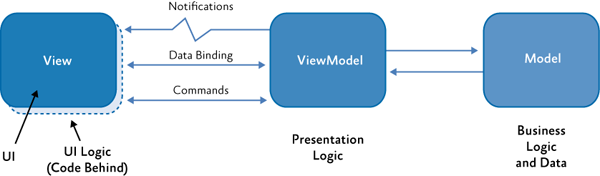
\includegraphics[width=\textwidth]{img/mvvm}
	\end{figure}
\end{frame}

\begin{frame}
	\frametitle{Zalety wzorca MVVM}
	\begin{itemize}
		\item
			W prosty sposób możemy tworzyć skomplikowane widoki
		\item
			Łatwy sposób testowania UI (testujemy ViewModel)
		\item
			Templating - prosty sposób na ponowne wykorzystanie elementów UI
	\end{itemize}
\end{frame}

%------------------------------------------------

\section{Biblioteka KnockoutJS}

\begin{frame}
	\frametitle{Biblioteka KnockoutJS}
	\begin{figure}
		\centering
		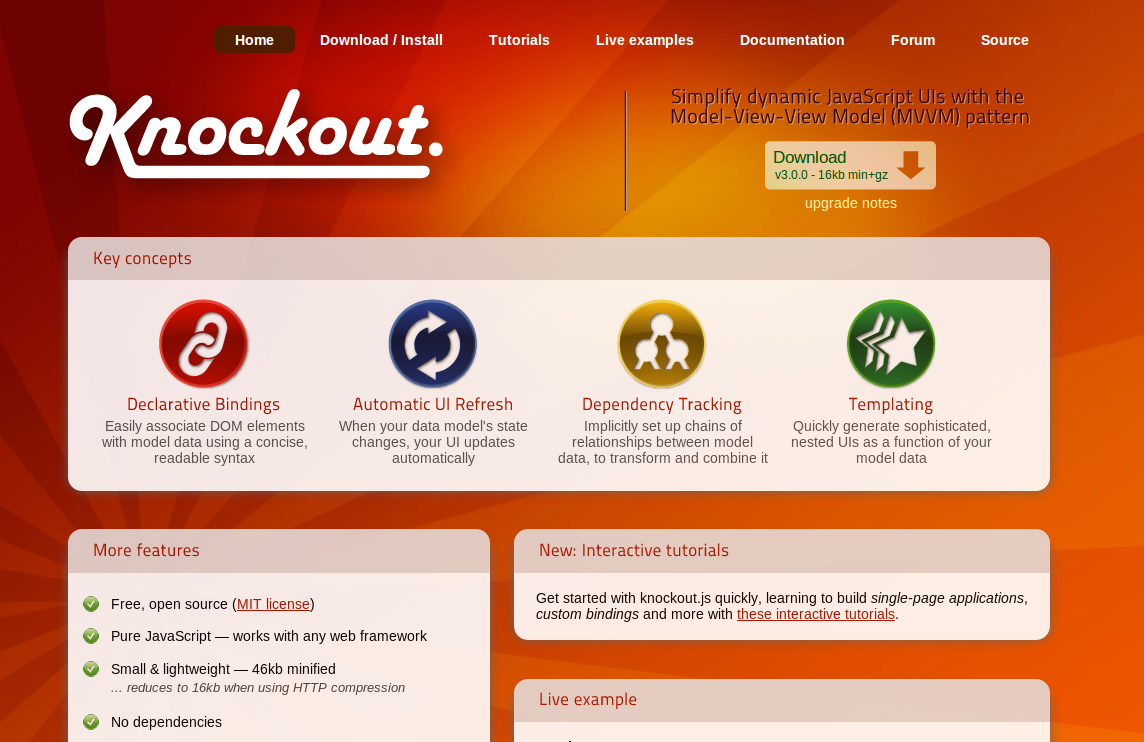
\includegraphics[width=\textwidth]{img/ko_page}
	\end{figure}
\end{frame}

\begin{frame}
	\Huge{\centerline{KnockoutJS Demo}}
	\begin{figure}
		\centering
		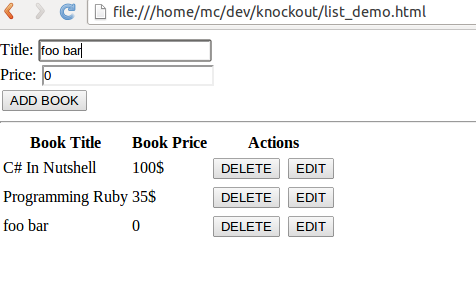
\includegraphics[width=\textwidth]{img/demo}
	\end{figure}
\end{frame}

\begin{frame}
	\frametitle{Subscribable type hierarchy}
	\begin{figure}
		\centering
		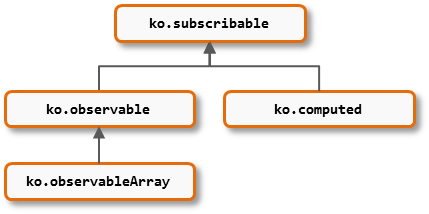
\includegraphics[width=\textwidth]{img/type-hierarchy}
	\end{figure}
\end{frame}

\begin{frame}
	\frametitle{mapper, pluginy itp.}
	
	\begin{itemize}
		\item
			mapping plugin (mapowanie pomiędzy observable i JSON)
		\item
			Dużo wtyczek pisanych przez społeczność (github)
	\end{itemize}
\end{frame}

%------------------------------------------------

\section{Zakończenie}

\begin{frame}
	\frametitle{Materiały}
	\begin{itemize}
		\item
			\url{http://knockoutjs.com/} (oficjalna strona biblioteki)
		\item
			\url{http://www.knockmeout.net/} (blog rniemeyer)
		\item
			\url{http://blog.stevensanderson.com/} (blog Steven~Sanderson)
		\item
			KnockoutJS Starter, \textit{Eric M. Barnard}, PACKT PUBLISHING 
			(ultra krótka - zaledwie 50 stron)
	\end{itemize}
\end{frame}

%------------------------------------------------

\begin{frame}
	\begin{figure}
		\centering
		
\includegraphics[width=4cm]{img/coding_horror}
	\end{figure}
	\Huge{\centerline{Uwagi? Pytania?}}
\end{frame}

%----------------------------------------------------------------------------------------

\end{document} 